\section{实测结果}\label{sec:eval}

\subsection{共包容量、同 IQ 包内偏移与状态机回放核验}\label{sec:eval_p2}

在 \texttt{R0} 馈线稳定链路上，表~\ref{tab:budget} 汇总的 10 个代表性布局与模式分支（轮次 2702--2710、2718）均实现 $10/10$ 计划任务双链独立完整恢复与逐字节校验通过。其中，\modejc{} 在单个次信道 PDU 中成功承载了 A 点 $26/26$\,B（载荷 \SI{179}{B}）、B 点 $52/26$\,B（载荷 \SI{205}{B}）与 C 点 $28/32$\,B（BlueBee 映射区扩展至 \SI{160}{B}，次信道载荷 \SI{205}{B}）三组完整双侧记录；B1 点（轮次 2710，$27/26$\,B）核验了 \modelc{} 单帧 \SI{27}{B} 直接承载边界（单尝试代理 \SI{1464}{\micro\second}），而 C 点（2709，30 片重组 10 条）与 B 点（2706，50 片重组 10 条）核验了 \fragproto{} 三片与五片空口重组。将 A（2704）、B（2718）、C（2707）三轮实录的 \ble{} 原始 IQ 送入 \stdfour{} 解码链 \texttt{zigbee\_rx.py} 后，三轮均独立恢复 $10/10$ 条有效命令，同 IQ 采样起点差值依次为 \SIrange{400.00}{400.25}{\micro\second}（中位数 \SI{400.25}{\micro\second}）、\SIrange{608.00}{608.25}{\micro\second}（中位数 \SI{608.00}{\micro\second}）与 \SIrange{416.00}{416.25}{\micro\second}（中位数 \SI{416.25}{\micro\second}），与式~\eqref{eq:offset} 预测的 \SI{400}、\SI{608} 与 \SI{416}{\micro\second} 偏差均不超过 \SI{4}{Msps} 下的单个采样间隔（\SI{0.25}{\micro\second}）。该结果仅验证同一采样时钟下的包内字段相对位置，不构成两块 HackRF 跨设备绝对同步精度。

此外，在实录流离线故障注入回放（\texttt{uc1\_h6\_replay.py}）中，基于 2714 实录 100 片 \fragproto{} 分片的 $7/7$ 项边界测试（尾部坏 CRC 拒收、同槽冲突隔离、跨槽分片不混合、\texttt{pending}/\texttt{closed} 耗尽预留不变量及时间倒退告警）与基于 2715 双侧各 300 包的 $4/4$ 项状态机测试（未知参考界拒收定时处理、错配 $b{=}0$ 布局拒收、首尝试坏 CRC 经重发恢复及合法 CRC 参数冲突取消挂起任务）均全部通过。

% ============================================================
%  表 2（中文同步版）：与 ../tables/tab-p4-main.tex 数值 100% 同步
%  数据源：python/experiments/p5_freeze_20261124/{p5_p4_cells.csv, p5_p4_paired_blocks.csv}
% ============================================================
\begin{table*}[t]
\centering
\caption{36 轮交替区组无线确认性实验的计划尝试内联合命令解析率与单位波形代理成本（\num{3600} 项计划任务，部分缺失条件 \texttt{R1}）。}
\label{tab:p4_main}
\setlength{\tabcolsep}{2.4pt}
\footnotesize
\begin{tabular}{@{}llccccccc@{}}
\toprule
\textbf{条件} & \textbf{模式} & $K$ & \textbf{首次} & \textbf{三区组} & \textbf{合并} & \textbf{均值$\pm$SD} & \textbf{单位成本} & \textbf{配对差 $\modejc{}-\text{模式}$ (pp)} \\
 & & & ($/300$) & B1/B2/B3 & ($/300$) & (\%) & (\si{\micro\second}/任务) & B1/B2/B3 (均值; 95\% $t$-CI) \\
\midrule
\multirow{3}{*}{A $(0,0)$, $K{=}1$}
  & \modejc{}              & 1 & 205/300 & 63 / 78 / 64 & 205/300 & $68.3 \pm 8.4$  & \num{2411.7}  & --- \\
  & \modesc{}              & 1 & 212/300 & 66 / 81 / 65 & 212/300 & $70.7 \pm 9.0$  & \num{2332.1}  & $-3/{-}3/{-}1$（$-2.33$；$[-5.20, +0.54]$） \\
  & \modelc{}$^{\mathrm{a}}$ & 1 & 204/300 & 51 / 90 / 63 & 204/300 & $68.0 \pm 20.0$ & \num{2141.2}  & $+12/{-}12/{+}1$（$+0.33$；$[-29.51, +30.18]$） \\
\midrule
\multirow{3}{*}{A $(0,0)$, $Q{=}6000$}
  & \modejc{}              & 3 & 224/300 & 95 / 100 / 99  & 294/300 & $98.0 \pm 2.6$ & \num{5044.9}  & --- \\
  & \modesc{}              & 3 & 227/300 & 99 / 100 / 100 & 299/300 & $99.7 \pm 0.6$ & \num{4960.5}  & $-4/{+}0/{-}1$（$-1.67$；$[-6.84, +3.50]$） \\
  & \modelc{}$^{\mathrm{a}}$ & 4 & 201/300 & 99 / 100 / 96  & 295/300 & $98.3 \pm 2.1$ & \num{5922.7}  & $-4/{+}0/{+}3$（$-0.33$；$[-9.06, +8.39]$） \\
\midrule
\multirow{3}{*}{B $(26,0)$, $K{=}1$}
  & \modejc{}              & 1 & 238/300 & 72 / 86 / 80 & 238/300 & $79.3 \pm 7.0$  & \num{2339.5}  & --- \\
  & \modesc{}              & 1 & 216/300 & 75 / 78 / 63 & 216/300 & $72.0 \pm 7.9$  & \num{2577.8}  & $-3/{+}8/{+}17$（$+7.33$；$[-17.55, +32.22]$） \\
  & \modelc{}$^{\mathrm{a}}$ & 1 & 86/300  & 43 / 36 / 7  & 86/300  & $28.7 \pm 19.1$ & \num{10130.2} & $+29/{+}50/{+}73$（$+50.67$；$[-4.00, +105.34]^{\mathrm{b}}$） \\
\midrule
\multirow{3}{*}{B $(26,0)$, $Q{=}6000$}
  & \modejc{}              & 3 & 195/300 & 99 / 100 / 92 & 291/300 & $97.0 \pm 4.4$  & \num{5740.2}  & --- \\
  & \modesc{}              & 3 & 224/300 & 99 / 99 / 99  & 297/300 & $99.0 \pm 0.0$  & \num{5624.2}  & $+0/{+}1/{-}7$（$-2.00$；$[-12.83, +8.83]$） \\
  & \modelc{}$^{\mathrm{a}}$ & 2 & 56/300  & 76 / 0 / 17   & 93/300  & $31.0 \pm 39.9$ & \num{18735.5} & $+23/{+}100/{+}75$（$+66.00$；$[-31.58, +163.58]^{\mathrm{b}}$） \\
\bottomrule
\end{tabular}
\par\smallskip
\raggedright\scriptsize
每单元合并 $n{=}3$ 独立交替区组 $\times$ $100$ 计划任务（每单元 $300$ 项；四分类结果见图~\ref{fig:p4_tradeoff}a）。双侧在至多 $K$ 次计划尝试内均校验通过即计为联合解析（不含截止期前按时交付审计）；\modelc{} 须在单次尝试内集齐全部分片。每单元提交/未用波形代理（\si{\micro\second}）：A-$K{=}1$ \num{494400}/$0$（\modejc{},\modesc{}）、\num{436800}/$0$（\modelc{}）；A-$Q$ \num{1483200}/\num{316800}（\modejc{},\modesc{}）、\num{1747200}/\num{52800}（\modelc{}）；B-$K{=}1$ \num{556800}/$0$（\modejc{},\modesc{}）、\num{871200}/$0$（\modelc{}）；B-$Q$ \num{1670400}/\num{129600}（\modejc{},\modesc{}）、\num{1742400}/\num{57600}（\modelc{}；B2 轮次 2743 解析 $0/100$，单轮成本记 \texttt{N/A}）。$^{\mathrm{a}}$\modejc{}/\modesc{}：BLE ch3（\SI{2410}{MHz}）；\modelc{}：ch39（\SI{2480}{MHz}，配置级）。$^{\mathrm{b}}$$\text{df}{=}2$ $t$-CI（$t_{0.975,2}{=}4.303$）跨零并超出 $\pm 100$\,pp。
\end{table*}


\begin{figure*}[t]
  \centering
  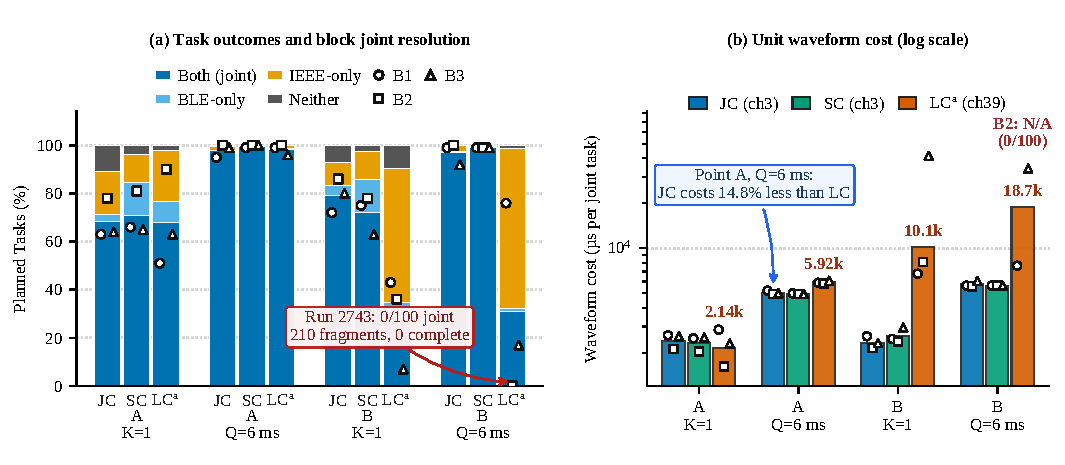
\includegraphics[width=\textwidth]{fig-p4-tradeoff.pdf}
  \caption{部分缺失无线条件 \texttt{R1} 下 36 轮确认性实验（\num{3600} 项计划任务）的四分类结果与单位波形代理成本（$K$ 为单任务计划尝试次数；$Q$ 为单任务波形预算上限，在 \SI{6000}{\micro\second} 下为 \modejc{}/\modesc{}/\modelc{}$^{\ast}$ 分别分配 A 点 $K{=}3/3/4$、B 点 $K{=}3/3/2$）：(a) 计划任务占比（\%），四分类堆叠柱分母为 $300$（合并三区组），B1/B2/B3 散点分母为 $100$（各区组独立比例；如 B 点同预算 \modelc{}$^{\ast}$ 合并联合成功柱为 $93/300$，三点依次为 $76/100$、$0/100$、$17/100$）；(b) 单位联合成功任务提交波形代理成本（对数坐标；柱为三区组总提交波形成本除以总联合成功任务数，点为各区组单轮单位成本；B2 轮次 2743 因零成功单轮记 \texttt{N/A}，其提交成本仍计入合并分子，三区组合并单位成本为 \SI{18735.5}{\micro\second}/联合成功任务；\modelc{}$^{\ast}$ 使用 \ble{} ch39，\modejc{}/\modesc{} 使用 ch3）。}
  \label{fig:p4_tradeoff}
\end{figure*}

\subsection{部分缺失无线条件 \texttt{R1} 下的成本与联合解析权衡}\label{sec:eval_p4}

P4 全部 36 轮确认性实验（\num{3600} 项计划任务）均通过采集与一致性门禁核验：全部接收摘要状态为 \texttt{complete}，队列溢出总数为 $0$，最大削波占比为 $0.00$，板端提交完成率 $100\%$ 且失败数为 $0$，全部 12 份跨模式比较记录均满足配置一致。表~\ref{tab:p4_main} 与图~\ref{fig:p4_tradeoff} 汇总了 12 个条件单元的计划尝试内联合解析率、四分类分布及单位成功任务波形代理成本。

\textbf{短负载 A 点（$b{=}0, z{=}0$，传统广播无需分片）：}如表~\ref{tab:budget} 所示，无需分片的 \modelc{} 单次尝试波形代理最低（\SI{1456}{\micro\second}，\modejc{}/\modesc{} 为 \SI{1648}{\micro\second}）。在单次尝试（$K{=}1$）条件下，三模式合并联合解析率接近（\modejc{} $68.3\%$ 即 $205/300$，\modesc{} $70.7\%$ 即 $212/300$，\modelc{} $68.0\%$ 即 $204/300$），因此 \modelc{} 取得最低的合并单位成功成本（\SI{2141.2}{\micro\second}/任务，低于 \modesc{} 的 \SI{2332.1} 与 \modejc{} 的 \SI{2411.7}{\micro\second}/任务）。然而在同预算上限 $Q{=}\SI{6000}{\micro\second}$ 下（\modejc{}/\modesc{} 分配 $K{=}3$，\modelc{} 分配 $K{=}4$），三模式计划尝试内联合解析率均逼近饱和（\modejc{} $98.0\%$、\modesc{} $99.7\%$、\modelc{} $98.3\%$）；由于开环 \modelc{} 仍为全部任务消耗了第 $4$ 次尝试（总提交 \SI{1747200}{\micro\second}，仅余 \SI{52800}{\micro\second} 未用预算），而 \modejc{}/\modesc{} 在 $K{=}3$（总提交 \SI{1483200}{\micro\second}，保留 \SI{316800}{\micro\second} 未用预算）下已接近全收，单位成功任务成本排序随策略发生翻转：\modejc{}（\SI{5044.9}{\micro\second}/任务）与 \modesc{}（\SI{4960.5}{\micro\second}/任务）分别比 \modelc{}（\SI{5922.7}{\micro\second}/任务）低约 $14.8\%$ 与 $16.2\%$（图~\ref{fig:p4_tradeoff}(b)）。

\textbf{长负载 B 点（$b{=}26, z{=}0$，结构差异与无线观测）：}从协议结构看，面对 \SI{52}{B} \ble{} 记录，\modejc{} 与 \modesc{} 仍以单个次信道数据单元完整承载（\SI{1856}{\micro\second}/尝试，$Q{=}\SI{6000}{\micro\second}$ 下分配 $K{=}3$），而 \modelc{} 须切分为 $5$ 片 \fragproto{} 分片（$6$ 突发、\SI{2904}{\micro\second}/尝试，同预算下被压缩至 $K{=}2$）。在所测 ch3 \modejc{} 对 ch39 \modelc{} 无线配置下，三个独立区组均观察到 \modejc{} 较高的联合解析率：$K{=}1$ 时 \modejc{} 均值 $79.3\%$（$238/300$）对比 \modelc{} $28.7\%$（$86/300$），逐区组差值为 $+29/+50/+73$\,pp（均值 $+50.67$\,pp，$95\%$ $t$ 区间 $[-4.00, +105.34]$\,pp），合并单位成功成本低 $76.9\%$（\SI{2339.5} vs.\ \SI{10130.2}{\micro\second}/任务）；$Q{=}\SI{6000}{\micro\second}$ 时 \modejc{} 均值 $97.0\%$（$291/300$）对比 \modelc{} $31.0\%$（$93/300$），逐区组差值为 $+23/+100/+75$\,pp（均值 $+66.00$\,pp，$95\%$ $t$ 区间 $[-31.58, +163.58]$\,pp），合并单位成功成本低 $69.4\%$（\SI{5740.2} vs.\ \SI{18735.5}{\micro\second}/任务）。必须指出两项边界：其一，受限于 $n{=}3$ 区组（$\text{df}{=}2$）小样本 $t$ 近似与区组间大幅波动，两项置信区间均跨零且端点超出 $\pm 100$\,pp，因此不宣称统计显著；其二，由于 \modejc{}/\modesc{} 使用 ch3 而 \modelc{} 使用 ch39，上述差距严格限定于所测封装与信道组合，不能单独归因于格式。分片级记录直观揭示了完成条件的苛刻性（图~\ref{fig:p4_tradeoff}(a)）：在 B2 轮次 2743（\modelc{}，$Q{=}\SI{6000}{\micro\second}$，$K{=}2$）中，\stdfour{} 侧独立恢复 $98/100$ 项任务，\ble{} 侧共收到 $210$ 个有效 \fragproto{} 分片，但无任何一次尝试集齐全部五片，最终完整重组为 $0$（\texttt{zigbee\_only} $=98/100$，联合成功 $0/100$，单轮单位成本 \texttt{N/A}）；B3 轮次 2761 与 2764 分别收到 $306$ 与 $615$ 片，但仅完整重组 $9$ 与 $19$ 条（联合成功 $7/100$ 与 $17/100$）。现有日志无法识别单个分片缺失的具体物理成因；若用 $p^5$ 刻画重组概率，还需额外假设五片接收相互独立且成功概率相同。

\textbf{同频公平对照（\modejc{} 对 \modesc{}）：}在相同频点（\ble{} ch3、\stdfour{} ch12，$12/12$ 满足协议归因检查）下，四组条件的 $\modejc{}-\modesc{}$ 均值差依次为 A-$K{=}1$ $-2.33$\,pp（$[-5.20, +0.54]$）、A-$Q$ $-1.67$\,pp（$[-6.84, +3.50]$）、B-$K{=}1$ $+7.33$\,pp（$[-17.55, +32.22]$）与 B-$Q$ $-2.00$\,pp（$[-12.83, +8.83]$），置信区间均跨零。在已测条件下，三个区组未显示 \modejc{} 相对 \modesc{} 稳定的联合解析优势（配置匹配与区间跨零均不能证明两者统计等效）。从四分类描述性分布看（图~\ref{fig:p4_tradeoff}(a)），$K{=}1$ 合并 300 项任务中，\modejc{} 呈现更少的 \texttt{ble\_only} 与更多的共同缺失 \texttt{neither}——A 点 \modejc{} 为 $9/300$ 与 $33/300$，而 \modesc{} 为 $42/300$ 与 $12/300$；B 点 \modejc{} 为 $12/300$ 与 $21/300$，而 \modesc{} 为 $41/300$ 与 $8/300$（本文不对双侧相关性作形式假设检验），这一形态与共享或分离次信道射频突发的结构一致。由此，\modejc{} 相对同频 \modesc{} 可直接确认的结构收益在于：在相等的单次尝试提交波形代理预算下将突发数由 $3$ 次减至 $2$ 次，并提供经同 IQ 核验的固定包内位置偏移以支撑共包时间参考。

% ============================================================
%  表 III（中文伴生版）：与 ../tables/tab-p2-time.tex 数值 100% 同步
%  数据源：python/experiments/p5_freeze_20261124/p5_p2_h5.csv
% ============================================================
\begin{table}[t]
\centering
\caption{固定次信道时间参考留出残差与单侧馈线断开恢复实例（轮次 2715--2717，\texttt{time} 配置）}
\label{tab:p2_time}
\setlength{\tabcolsep}{1.2pt}
\scriptsize
\begin{tabular}{@{}llccccccc@{}}
\toprule
\textbf{轮} & \textbf{场景} & \textbf{联合} & \multicolumn{2}{c}{\textbf{覆盖}} & \multicolumn{2}{c}{\textbf{计划内恢复}} & \multicolumn{2}{c}{\textbf{中位/P95 (ms)}} \\
\cmidrule(lr){4-5}\cmidrule(lr){6-7}\cmidrule(lr){8-9}
 & & 任务 & B & Z & B & Z & B & Z \\
\midrule
2715 & 正常   & 6/6 & 24/24 & 24/24 & N/A(0/0) & N/A(0/0) & .223/.318 & .129/.295 \\
2716 & B断馈  & 5/6 & 19/24 & 24/24 & 1/1      & N/A(0/0) & .242/.395 & .144/.330 \\
2717 & Z断馈  & 5/6 & 24/24 & 19/24 & N/A(0/0) & 1/1      & .222/.317 & .134/.336 \\
\bottomrule
\end{tabular}
\par\smallskip
\raggedright\scriptsize
三轮均采用 \texttt{R0} 馈线直连拓扑，每轮 $300$ 槽（周期 \SI{500}{ms}：$6$ 项任务 $\times$ $K{=}3$ 与 $282$ 个等长纯时间更新槽；双侧共覆盖探针的估计差中位数为 \SIrange{0.140}{0.153}{ms}、P95 为 \SIrange{0.202}{0.264}{ms}，$n{=}24,19,19$）。按 \texttt{uc1\_time\_tail\_audit} 口径将停发后尾段 \texttt{stale}（双侧各 $1/1$）与计划内事件分离；未受干预侧无计划内失更事件，记为 \texttt{N/A (0/0)}。每轮均有 $0/6$ 项计划任务通过定时软件处理判定（外部射频参考界未校准）。表中数据为本侧 IQ 采样域留出绝对预测误差，不代表跨设备时钟同步精度。
\end{table}


\subsection{固定次信道时间参考与单侧馈线断开恢复}\label{sec:eval_time}

表~\ref{tab:p2_time} 给出了 \texttt{R0} 馈线直连拓扑下三轮 \texttt{time} 配置（B 点 \modejc{}，每轮 $300$ 槽含 $282$ 个等长纯时间更新槽，按 \texttt{uc1\_time\_tail\_audit} 口径将停发后录制尾段 \texttt{stale} 与计划内事件分离）的观测结果。无干预基线（轮次 2715）中，双侧联合解析 $6/6$ 项任务且留出时间探针覆盖均为 $24/24$，\ble{} 与 \stdfour{} 本侧 IQ 采样域绝对预测残差中位数分别为 \SI{0.223}{ms}（P95 \SI{0.318}{ms}）与 \SI{0.129}{ms}（P95 \SI{0.295}{ms}）。在轮次 2716（人工断开 \ble{} 侧馈线）与 2717（人工断开 \stdfour{} 侧馈线）中，现场笔记记录了人工干预的大致包序范围；未受干预侧始终维持 $24/24$ 留出探针覆盖且计划内失更事件为 $0$ 次（恢复率记 \texttt{N/A (0/0)}）；在断开馈线与恢复接收的过程中，受干预侧先后出现 \texttt{holdover}、\texttt{stale}、\texttt{reacquiring} 与 \texttt{tracking}，各取得 $1/1$ 计划内恢复（留出探针覆盖 $19/24$，联合任务 $5/6$）。按受干预接收机本侧 IQ 采样索引计时，从进入 \texttt{stale} 至恢复 \texttt{tracking} 的时长在 2716（\ble{} 侧）与 2717（\stdfour{} 侧）分别为 \SI{23.0}{s}（\SI{23003.1}{ms}）与 \SI{24.0}{s}（\SI{24002.6}{ms}）；其中，重获训练（从首次进入 \texttt{reacquiring} 至恢复 \texttt{tracking}，每轮均收集 $8$ 个训练包）分别耗时约 \SI{7.0}{s}（\SI{6996.0}{ms}）与 \SI{9.0}{s}（\SI{8994.8}{ms}）。三轮实验的定时处理均因缺少外部校准参考界而保守拒绝（$0/6$）。上述数据作为共包时间参考机制的可用性与失更恢复功能实例，不与 X-Sync~\cite{hofmann2021xsync} 等跨设备绝对同步精度直接对比。
